% vim: set foldmethod=marker foldlevel=0:

\documentclass[a4paper]{article}
\usepackage[UKenglish]{babel}

\usepackage{preamble}

\usepackage{graphicx}
\graphicspath{ {./imgs/} }

\fancyhead[L]{MA146 Assignment 4}
\title{MA146 Methods of Mathematical Modelling 1, Assignment 4}
\colorlet{questionbodycolor}{green!50!teal!50}

\begin{document}

\maketitle

\setlength{\parindent}{0em}
\setlength{\parskip}{1em}

% {{{ Q2
\question{2}

\begin{questionbody}
The motion of a particle in a viscous, resistive medium can lead to the (already nondimensional) initial value problem \[
\diff t v(t) = -v(t) + \varepsilon v(t)^2, \quad t > 0, \quad v(0) = 1,
\] where $\varepsilon \in (0, 1)$ is a \enquote{small} parameter.
\end{questionbody}

\subsection{~} % 2.a

\begin{questionbody}
Find the solution to the initial value problem, for instance, by using a suitable substitution of the dependent variable.
\end{questionbody}

I have no idea what substitution to use, sorry.

\subsection{~} % 2.b

\begin{questionbody}
Consider now the ansatz $v(t) = v_0(t) + \varepsilon v_1(t)$ and substitute it into the initial value problem. Dropping all terms with $\varepsilon^p$ where $p \ge 2$ (these are deemed \enquote{small}), derive and solve initial value problems for $v_0$ and $v_1$.
\end{questionbody}

Consider $v(t) = v_0(t) + \varepsilon v_1(t)$. Then \begin{align*}
	\diff t v(t) &= \diff t v_0(t) + \varepsilon \diff t v_1(t)\\[1ex]
				 &= -v_0(t) - \varepsilon v_1(t) + \varepsilon \l(v_0(t)^2 + 2 \varepsilon v_0(t) v_1(t) + \varepsilon^2 v_1(t)^2 \r)\\[1ex]
				 &= -v_0(t) - \varepsilon v_1(t) + \varepsilon v_0(t)^2 + \cancelto{0}{\varepsilon^2 \l(\cdots\r)}\\[1ex]
	\therefore \diff t v_0(t) + \varepsilon \diff t v_1(t) &= -v_0(t) - \varepsilon v_1(t) + \varepsilon v_0(t)^2
\end{align*}

And the initial condition becomes $v_0(0) + \varepsilon v_1(0) = 1$. Unfortunately, I have no idea where to go from here.

\vspace{3em}
\begin{questionbody}
Remark: Using the approximation $(1 + \varepsilon z)^{-1} \approx 1 - \varepsilon z$ the two solutions can be related. This can help to check the result, no need to discuss it any further.
\end{questionbody}
% }}}

% {{{ Q3
\newquestion{3}

\subsection{~} % 3.a

\begin{questionbody}
Using the law of mass action, formulate the following reactions as differential equations: \[
3\text{K} + 4\text{M} \xrightleftharpoons[\ r_2\ ]{\ r_1\ } 2\text{A} + 6\text{B}
\]
\end{questionbody}

Let $k(t)$ be the concentration of K and likewise pairing $m(t)$ with M, $a(t)$ with A, and $b(t)$ with B. Then we get the following equations \begin{align*}
	\diff t k(t) &= -3 r_1 k(t) m(t) + 3 r_2 a(t) b(t)\\[1ex]
	\diff t m(t) &= -4 r_1 k(t) m(t) + 4 r_2 a(t) b(t)\\[1ex]
	\diff t a(t) &= 2 r_1 k(t) m(t) - 2 r_2 a(t) b(t)\\[1ex]
	\diff t b(t) &= 6 r_1 k(t) m(t) - 6 r_2 a(t) b(t)
\end{align*}

\subsection{~} % 3.b

\begin{questionbody}
Two nitrosyl chloride molecules can react to two nitric oxide and one chlorine molecules. This dissociation is an elementary chemical reaction.

Write it as a diagram (choosing any suitable letters for the molecules and the rate factor, precise chemical formulas are not required) and then as a system of differential equations to model the process.
\end{questionbody}

$$2\text{NOCl} \xrightarrow{\ k\ } 2\text{NO} + \text{Cl}_2$$

Let $s(t)$ be the concentration of nitrosyl chloride, $n(t)$ be the concentration of nitric oxide, and $c(t)$ be the concentration of chlorine. Then the rate equations are \begin{align*}
	\diff t s(t) &= -2ks(t)\\[1ex]
	\diff t n(t) &= 2ks(t)\\[1ex]
	\diff t c(t) &= ks(t)
\end{align*}

\subsection{~} % 3.c

\begin{questionbody}
Consider the following SIR model (a more basic model than the one discussed in the
lectures) for the spread of infectious diseases: \begin{align*}
\dd st (t) &= -\beta i(t) s(t), \\
\dd it (t) &= \beta i(t) s(t) - \gamma i(t), \\
\dd rt (t) &= \gamma i(t).
\end{align*}

Find a suitable \enquote{reaction} diagram (it may contain several \enquote{reactions}, which then are to be understood as coupled) such that the above system is obtained when the law of mass action is applied to it.
\end{questionbody}

$$S + I \xrightarrow{\ \beta\ } I \xrightarrow{\ \gamma\ } R$$
% }}}

% {{{ Q4
\newquestion{4}

\begin{questionbody}
Consider the system of linear first order equations \begin{equation*}
\begin{array}{l}
x_1'(t) = x_2(t) \\[0.5ex]
x_2'(t) = -c x_1(t) - b x_2(t)
\end{array}
\quad \Leftrightarrow \quad
\mathbf{x}'(t) = A \mathbf{x}(t) \quad\text{with } A = \begin{pmatrix} 0 & 1 \\ -c & -b \end{pmatrix}
\end{equation*}
\end{questionbody}

\subsection{~} % 4.a

\begin{questionbody}
Retrieve the Jupyter notebook \texttt{MA146\_Assignment4.ipynb}. The problem with $b = 0$ and $c = 16$ is implemented for the initial data $x_1(\pi) = 13$, $x_2(\pi) = 8$.

Consider now the parameters $b = −0.2$ and $c = 8$. Use the notebook to solve the system three times with initial data $x_1(0) \in \{1.5, 2.0, 2.7\}$ and always $x_2(0) = 0$.

Generate a parametric plot displaying all solutions for $t \in [0, 4\pi]$ (the template at the bottom of the notebook for this part indicates how one can plot several curves together).

Submit your code (the cell for this question is sufficient) and the graphics output.
\end{questionbody}

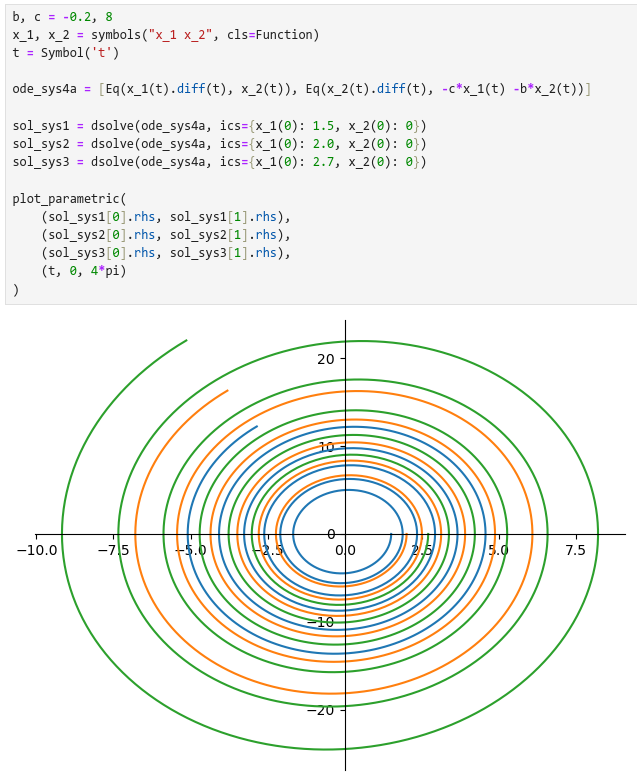
\includegraphics[scale=0.55]{Q4}

\subsection{~} % 4.b

\begin{questionbody}
How is the system of differential equations related to the problems in Question 2 of Assignment 1?
\end{questionbody}

Assignment 1 question 2 was about the differential equation $$a \f{\d^2}{\d t^2}x(t) + b \diff t x(t) + cx(t) = 0$$

The system \begin{align*}
	x_1'(t) &= x_2(t)\\[1ex]
	x_2'(t) &= -c x_1(t) - b x_2(t)
\end{align*}is related in that we can imagine $x_1(t) = x(t)$ and $\ds x_2(t) = \diff t x(t)$. Then the system becomes \begin{align*}
	\diff t x(t)          &= \diff t x(t)\\[1ex]
	\f{\d^2}{\d t^2} x(t) &= -c x(t) - b \diff t x(t)
\end{align*}

The first line is just obviously always true, and the second line is equivalent to the differential equation given in assignment 1 question 2, just with $b$ and $c$ scaled to make $a=1$.
% }}}

\end{document}
